%con este comando quitamos las identaciones
\setlength{\parindent}{0pt}
\documentclass[10pt,a4paper]{article}
\usepackage[utf8]{inputenc}
\usepackage{amsmath}
\usepackage{amsfonts}
\usepackage{amssymb}
\usepackage{graphicx}
\usepackage[left=2cm,right=2cm,top=2cm,bottom=2cm]{geometry}
\usepackage{graphicx}
\usepackage{subcaption}


\title{Informe Tarea 1 - M\'etodos Num\'ericos}
\author{Bruno Quezada}
\date{27 de septiembre}
\begin{document}
\maketitle

\vspace{17cm}
\begin{flushright}
\textbf{Asignatura:} Métodos Numéricos - FI 3104-1\\
\textbf{Profesor Cátedra:} Valentino González\\
\textbf{Auxiliares:} José Vines, Jou-Hui Ho \\
\end{flushright}
\pagebreak

\section{Pregunta 1}
\noindent
\subsection{Introducción}

%Ac´a introduzco el problema a resolver, par´ametros como las condiciones de borde,
%etc. Recuerden incluir toda la informaci´on necesaria para que alguien pueda
%reproducir su programa/resultados leyendo su informe - pero sean concisos, lo
%mejor es una explicaci´on corta y clara.

En esta pregunta se busca comparar dos métodos de interpolación de datos, utilizando métodos que pasen por todos los puntos entregados. Se comparará el método de spline: spl.InterpolatedUnivariateSpline() y el método de los polinomios de Lagrange. Para evaluar la interpolación se comparará como se ajustan las curvas de ambos métodos a un muestreo de la función:\\
\begin{center}
$f(x) = \dfrac{1}{1 + 25x^2}$\\
\end{center}
En el intervalo $[-1,1]$ para un número variable de puntos en este intervalo.



\subsection{Procedimiento}
El objetivo es crear una función que calcule el polinomio de Lagrange para ajustar algún vector de datos, para ello, se siguieron múltiples pasos. En primer lugar, se creó la función\textit{ lagrange(x,y,X)} la cual a partir de los datos en $x$ e $y$ calculaba la interpolación de la curva en el punto $X$. Si bien esta función cumple el objetivo, no es una solución eficiente, porque calcula el polinomio de Lagrange para cada punto que se quiera interpolar, independiente de si el vector de datos es siempre el mismo. Por ello, se busca una solución que devuelva el polinomio y no un valor, para ello es necesario construir una función que retorne funciones. Para proceder, primero se decide afrontar un problema un poco más fácil: se crea la función \textit{aux(x)} la cual retorna funciones y se estudia su comportamiento. Por último, con los nuevos conocimientos adquiridos se puede generar la función \textit{pol\textunderscore lagrange(x,y)}, la cual retorna el polinomio de Lagrange que ajusta los datos entregados. Con esta función se puede generar el polinomio de Lagrenge que ajusta los datos\\

\noindent En el caso de \textit{spline}, se recurre a la función \textit{InterpolatedUnivariateSpline()} del módulo \textit{scipy.interpolate}. Las interpolaciones del tipo \textit{spline} consideran una partición del dominio en el que se quiere interpolar para ajustar cada trozo con un polinomio, imponiendo condiciones sobre la función y sus derivadas se logra obtener una interpolación que pasa por los puntos y que es suave. En este caso el índice de suavidad se le puede ajustar, lo que controla las condiciones que se le impone a la interpolación.

\subsection{Resultados}
en las figuras \ref{fig8} a \ref{fig100} se encuentran los resultados de ambas interpolaciones para 8, 12, 40 y 100 puntos de $f(x)$.\\


\begin{figure}[h]
    \centering
    \begin{subfigure}[h]{0.4\textwidth}
        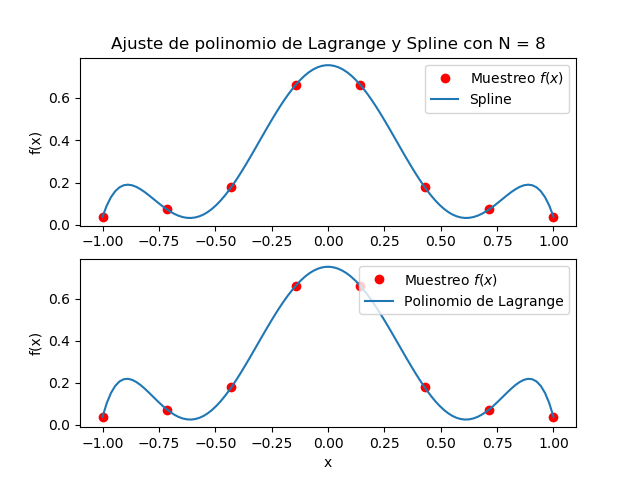
\includegraphics[width=\textwidth]{ajuste8.png}
        \caption{Ajuste de polinomio de Lagrange y spline con 8 puntos a interpolar}
        \label{fig8} 
    \end{subfigure}
    ~ %add desired spacing between images, e. g. ~, \quad, \qquad, \hfill etc. 
      %(or a blank line to force the subfigure onto a new line)
    \begin{subfigure}[h]{0.4\textwidth}
        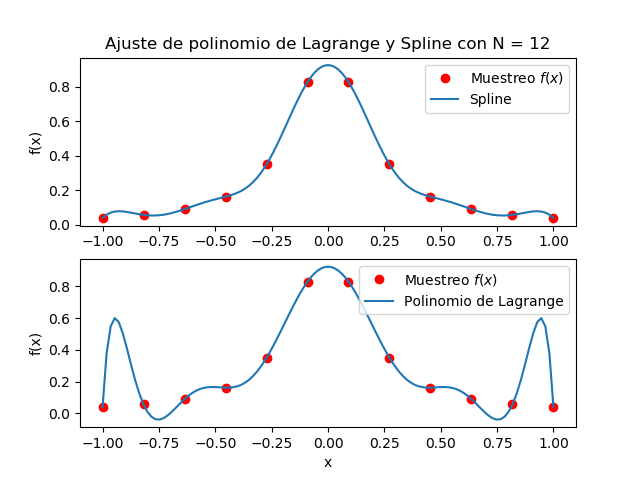
\includegraphics[width=\textwidth]{ajuste12.png}
        \caption{Ajuste de polinomio de Lagrange y spline con 12 puntos a interpolar}
    \end{subfigure}
    \begin{subfigure}[h]{0.4\textwidth}
        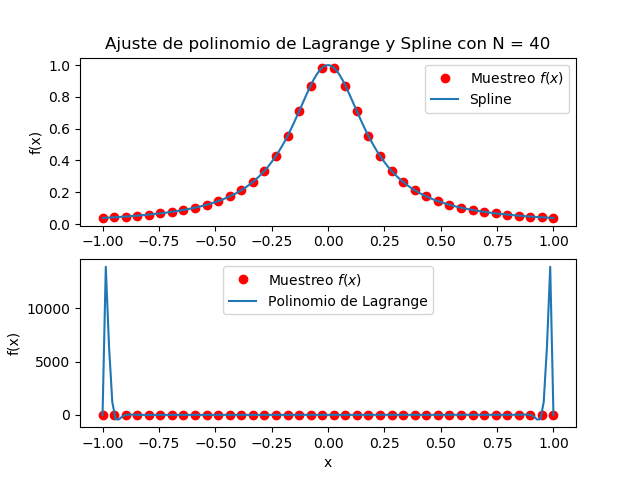
\includegraphics[width=\textwidth]{ajuste40.png}
        \caption{Ajuste de polinomio de Lagrange y spline con 40 puntos a interpolar}
    \end{subfigure}
    ~ %add desired spacing between images, e. g. ~, \quad, \qquad, \hfill etc. 
      %(or a blank line to force the subfigure onto a new line)
    \begin{subfigure}[h]{0.4\textwidth}
        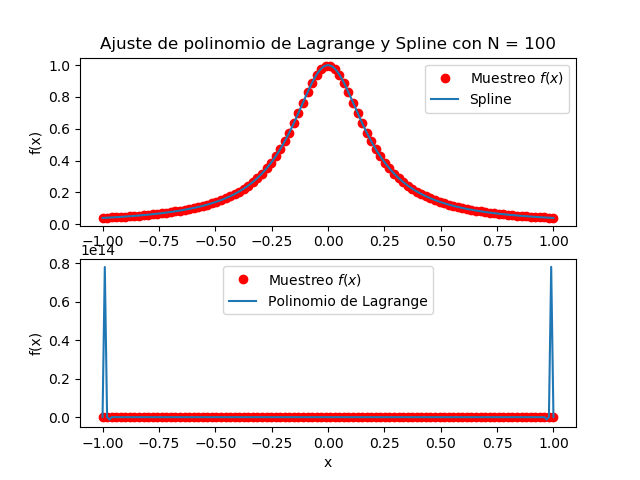
\includegraphics[width=\textwidth]{ajuste100.png}
        \caption{Ajuste de polinomio de Lagrange y spline con 100 puntos a interpolar}
        \label{fig100}
    \end{subfigure}
\end{figure}

\subsection{Análisis y Conclusiones}
Se puede observar claramente que a medida que aumentan los puntos a interpolar la función \textit{pol\textunderscore lagrange()}la función empieza a perder suavidad, llegando al caso extremo en la figura \ref{fig100} en donde el valor de la interpolación toma valores del orden de $10^{14}$ cerca de los bordes. Por inspección, se observa que al aumentar los puntos a más de $\approx 12$ la interpolación a través de Lagrange para $f(x)$ empieza a perder suavidad y las soluciones dejan de ser razonables. En cambio, para la función de \textit{spline()}, la suavidad de la función se mantiene a pesar de aumentar el número de puntos.\\

Debido a lo anterior se considera que ajustar a través de una \textit{spline} se llega a una solución más adecuada, a pesar de que ambos métodos pueden ajustar, debido a la poca suavidad que presenta el método del polinomio de Lagrange al aumentar el número de puntos.\\

También se considera que se adquirió un conocimiento muy importante que es manejar funciones que retornen funciones, lo cual me permitirá obtener soluciones más generales para problemas de tipo numéricos.

\newpage
\section{Pregunta 2}

\subsection{Introducción}
Para esta pregunta se solicita emplear algoritmos de interpolación para estimar la anomalía climática experimentada en el 2011 a partir de los datos de anomalías históricas entre 2008 y 2017, excluyendo el 2011.\\

\subsection{Procedimiento}
En primer lugar es necesario importar los datos entregados a python. Como las capacidades intelectuales del autor no consiguieron  encontrar una solución elegante, se procedió a convertir el archivo .csv en uno .txt y utilizando el editor se removieron fácilmente las comas separadoras de los datos. Para importar los datos desde el .txt se utilizó la función \textit{loadtext()} de la librería \textit{numpy}.\\
Una vez importados los datos se generaron los vectores \textit{años} y \textit{anomalías}, los cuales contenían los datos necesarios para realizar la interpolación, con estos vectores se llamó a la función \textit{InterpolatedUnivariateSpline()} del módulo \textit{scipy.interpolate} y se estimaron los valores de las anomalías del 2011 y 2018.


\subsection{Resultados}
En la figura \ref{anomali}, se aprecia la interpolación de los datos generada por la función spline \textit{InterpolatedUnivariateSpline()}.\\
El valor interpolado de anomalía del 2011 es $0.66[C]$ por lo que hay un error de ajuste de $0.080[C]$ y la predicción para el 2018 es de $0.389[C]$

\begin{figure}[h]
\centering
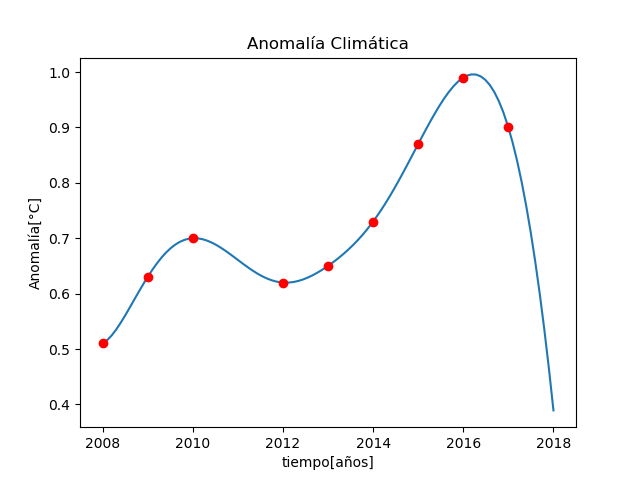
\includegraphics[scale=0.5]{interpolacion_anomalia.png}
\caption{Interpolación de la anomalía climática entre 2011 y 2018, para datos anuales entregados, a excepción del 2011}
\label{anomali}
\end{figure}



\subsection{Análisis y Conclusiones}
Considerando que el sistema climático es altamente caótico y, por lo tanto, muy difícil de predecir la estimación a través de interpolaciones no debe considerarse un proceso serio, sino solo pedagógico.\\
Hecha esta consideración la interpolación llega a un dato que se considera regular, ya que está dentro de los órdenes de magnitud esperados, pero que al considerar su significancia física se sabe que cada décima de grado de anomalía es una cantidad de energía tremenda en el planeta.\\
En el caso particular de esta interpolación, se puede observar que para las predicciones futuras la anomalía climática baja abruptamente, esto claramente se lo atribuye al carácter meramente matemático del algoritmo y se considera un resultado inválido.\\
Se considera que los métodos de interpolación son poderosos y que permiten extender el conocimiento que otorgan los datos de nuestras mediciones, pero que deben tomarse con cuidado, ya que no siempre es válido pensar que una interpolación, la cual sólo se basa en los datos entregados y no en las características físicas del problemas que se busca resolver, tiene una validez predictiva en todos los casos.\\
En el caso particular de la spline se considera una gran herramienta, ya que se puede ajustar su suavidad, por lo que las soluciones son menos propensas a tomar valores fuera del rango esperado, como con el caso del polinomio de Lagrange.
\end{document}
